\documentclass[conference]{IEEEtran}

\usepackage{graphicx}
\usepackage{amsmath}
\usepackage{amssymb}
\usepackage{cite}
\usepackage{hyperref}
\usepackage{booktabs}
\usepackage{multirow}
\usepackage{array}
\usepackage{algorithm}
\usepackage{algorithmic}
\usepackage{textcomp}
\usepackage{xcolor}
\usepackage{float}
\usepackage{tikz}
\usetikzlibrary{shapes.geometric, arrows.meta, positioning, fit, calc, backgrounds}

\hypersetup{
    colorlinks=true,
    linkcolor=black,
    citecolor=black,
    urlcolor=blue
}

\begin{document}

\title{Software Cost Estimation in Agile Methodology\\Using Deep Learning with Uncertainty Quantification}

\author{
\IEEEauthorblockN{Dr.~V.~Venkataiah}
\IEEEauthorblockA{
Associate Professor\\
Department of Computer Science \& Engineering\\
CMR College of Engineering \& Technology\\
Hyderabad, India
}
\and
\IEEEauthorblockN{
B.~Varshini\IEEEauthorrefmark{1},
B.~Sai~Manikanta~Karthik\IEEEauthorrefmark{2},
Ch.~Nava~Chaithanyaa\IEEEauthorrefmark{3}
}
\IEEEauthorblockA{
Department of Computer Science \& Engineering\\
CMR College of Engineering \& Technology (UGC Autonomous)\\
Affiliated to JNTUH, NAAC Accredited with A+ Grade\\
Kandlakoya, Medchal Road, Hyderabad -- 501401, India\\
}
}

\maketitle

\begin{abstract}
Predicting the total cost of a software project before it wraps up has never been straightforward, and the problem only gets harder under Agile workflows where scope evolves with every sprint cycle. Legacy formulas like COCOMO and Function Point Analysis assume a fixed-scope, plan-driven world and therefore miss the wealth of qualitative detail embedded in sprint retrospectives, standup notes, and backlog descriptions. In this study we put forward a deep learning pipeline that reads raw Agile project reports alongside structured project metadata, producing two simultaneous outputs: a dollar-valued cost forecast and a calibrated measure of how much that forecast should be trusted. The text branch relies on a BERT-Large encoder whose CLS representation is concatenated with an eighteen-feature numerical embedding generated by a small feedforward network; the fused vector then splits into a mean-prediction head and a variance-prediction head, both trained under a Gaussian negative-log-likelihood criterion. At inference time, twenty stochastic forward passes with active dropout decompose prediction uncertainty into a data-inherent (aleatoric) portion and a model-knowledge (epistemic) portion, enabling 90\% confidence bands around every estimate. We adopt a two-stage learning schedule that first locks the language encoder and trains only the regression layers, then unlocks everything with carefully separated learning rates, finishing in under ten minutes on a single H200 accelerator. Evaluated on a purpose-built collection of ten thousand synthetic yet realistic Agile reports spanning eight industry sectors, the system achieves an R\textsuperscript{2} of 0.9876 and a mean absolute percentage error of 6.71\%, cutting the best tree-ensemble baseline's error by more than half while simultaneously delivering actionable confidence intervals that point-estimate-only methods cannot provide.
\end{abstract}

\begin{IEEEkeywords}
Software cost estimation, Agile methodology, deep learning, BERT, uncertainty quantification, natural language processing
\end{IEEEkeywords}

% ════════════════════════════════════════════════════════════
\section{Introduction}
% ════════════════════════════════════════════════════════════

Few early-stage decisions shape a software initiative's outcome as decisively as its initial cost estimate. When that number is too low, teams face budget overruns, compressed timelines, and the kind of corner-cutting that breeds technical debt; when it is too high, viable projects never get funded. Industry-wide data paints a sobering picture: the Standish Group has reported year after year that upwards of two-thirds of software undertakings exceed their planned budgets, with poor estimation ranking among the top root causes \cite{standish2020}.

Agile development adds a distinctive layer of difficulty. The Scrum Guide \cite{schwaber2020} explicitly welcomes requirement changes even late in the development cycle, which means that the scope a team is estimating today may look entirely different by the third or fourth sprint. Classical cost formulas---Boehm's COCOMO \cite{boehm1981}, Putnam's SLIM \cite{putnam1978}, Albrecht and Gaffney's Function Point counting \cite{albrecht1979}---were all designed around the assumption that scope, staffing, and technology are settled before coding begins. That assumption simply does not hold in a Scrum environment where backlog refinement, sprint retrospectives, and daily standups continuously reshape both the work and the way it is performed. Usman et~al. \cite{usman2014} catalogued these mismatches in a broad literature survey and concluded that no parametric framework has yet earned convincing validation on Agile project data.

Over the past decade and a half, machine-learning researchers have tried to close the gap by training regression trees, support-vector machines, and shallow neural networks on historical effort datasets \cite{wen2012, sarro2016}. These learners outperform the parametric formulas, but two blind spots persist. First, virtually every published model works from a narrow table of numeric features---story points, headcount, velocity---while ignoring the detailed textual narratives that Agile teams produce in the normal course of their work. Second, not one of these systems tells the project manager how reliable its prediction actually is; the output is a bare number with no attached confidence.

Our work tackles both shortcomings at once. Specifically, we contribute:

\begin{itemize}
    \item \textbf{Multi-modal architecture:} We propose a deep learning model that fuses BERT-Large text embeddings from Agile project reports with structured numerical features through a late-fusion strategy, capturing both linguistic context and quantitative project characteristics.
    \item \textbf{Uncertainty quantification:} Our model produces dual outputs---a cost estimate and an associated uncertainty---trained via Gaussian Negative Log-Likelihood loss. Monte Carlo Dropout inference further decomposes the total uncertainty into aleatoric and epistemic components.
    \item \textbf{Two-phase training:} We introduce an efficient training strategy that first trains the regression head with a frozen BERT encoder, then fine-tunes the entire model with discriminative learning rates, achieving strong convergence in under 10 minutes on an NVIDIA H200 GPU.
    \item \textbf{Comprehensive evaluation:} We demonstrate that our approach achieves an R\textsuperscript{2} of 0.9876 and a MAPE of 6.71\% on 10,000 synthetic Agile project reports, substantially outperforming traditional machine learning baselines.
\end{itemize}

The remainder of this paper is organized as follows: Section~II reviews related work, Section~III describes the proposed methodology, Section~IV presents implementation details, Section~V discusses experimental results, Section~VI provides analysis and discussion, and Section~VII concludes with future directions.

% ════════════════════════════════════════════════════════════
\section{Literature Review}
% ════════════════════════════════════════════════════════════

Research on estimating the cost or effort of software projects stretches back roughly four decades, progressing through three recognizable phases: hand-tuned parametric formulas, statistical and ensemble learners, and---most recently---deep neural networks. Below we trace each phase and point out what remains unresolved.

\subsection{Traditional Parametric Models}

COCOMO, introduced by Boehm in the early 1980s \cite{boehm1981}, remains the single most referenced estimation framework in the literature. Its successor, COCOMO~II, traded raw lines-of-code counts for object points and function points, yet the core mechanism---a power-law relationship modulated by a handful of cost-driver multipliers---was never rethought for iterative lifecycles. Putnam's SLIM approach \cite{putnam1978} brought time dynamics into the picture by modeling staffing levels as a Rayleigh distribution, an idea that maps well onto multi-year government contracts but offers little traction for two-week sprints. Function Point Analysis, proposed by Albrecht and Gaffney \cite{albrecht1979}, decoupled size measurement from programming language, which was a practical advance; however, translating Agile user stories into function-point counts is notoriously subjective, as Usman et~al. \cite{usman2014} documented through an extensive survey of practitioner experiences.

\subsection{Machine Learning Approaches}

The early 2000s saw a wave of papers replacing parametric formulas with data-driven regressors. Wen et~al. \cite{wen2012} pulled together eighty-four of these studies and noted that neural networks and ensembles routinely topped classical regression, though margins were modest and depended heavily on which dataset was used. Sarro et~al. \cite{sarro2016} took a multi-objective view, simultaneously optimizing prediction accuracy and interval width on the ISBSG benchmark; their best configurations delivered MAPE figures in the low twenties.

Ensemble methods quickly became the default. Idri et~al. \cite{idri2016} benchmarked a range of ensemble configurations and found Gradient Boosting at the top, with a median relative error near 24.5\%. Pospieszny and colleagues \cite{pospieszny2018} pushed performance further by stacking multiple base estimators under a meta-learner, shaving eight to twelve additional percentage points off the error. A shared limitation of all these systems, however, is their exclusive reliance on tabular feature sets; none attempts to mine the natural-language records that Agile teams routinely generate.

\subsection{Deep Learning for Software Engineering}

The application of deep neural networks to software-engineering tasks accelerated once large pre-trained language models became widely available. Choetkiertikul et~al. \cite{choetkiertikul2019} trained a Long Short-Term Memory network to predict story-point assignments from issue-tracker text, with moderate success on publicly available open-source project data. Fu and Menzies \cite{fu2017} offered a cautionary result, demonstrating that well-tuned shallow models can rival deep networks when manual feature engineering is thorough---an observation that highlights the importance of text-level signals as the distinguishing advantage of deep architectures.

On the transformer side, BERT \cite{devlin2019} and its code-oriented descendant CodeBERT \cite{feng2020} have reshaped bug triage, commit classification, and requirement traceability in recent years. Sharma and Gupta \cite{sharma2022} explored plugging BERT embeddings into an effort-estimation pipeline, reaching R\textsuperscript{2} values near 0.85 on a JIRA-derived corpus. Their setup, though, processed text and metadata in separate streams without fusion, omitted any form of uncertainty output, and was evaluated on a single project domain.

\subsection{Uncertainty in Software Estimation}

Despite being the first question any budget holder asks---``how confident are you in that number?''---prediction confidence has received remarkably little attention in the cost-estimation community. Jorgensen's meta-analysis of expert surveys \cite{jorgensen2004} showed that human estimators produce badly miscalibrated intervals, a finding reinforced by Molokken-Ostvold and Jorgensen \cite{molokken2003}. On the modelling side, Mittas and Angelis \cite{mittas2013} proposed bootstrap-based confidence bands but acknowledged that bootstrapping captures sampling variability only, not the structural uncertainty that accumulates when a model encounters a project type it has rarely seen.

Gal and Ghahramani \cite{gal2016} showed that simply keeping dropout active during inference turns any dropout-trained network into an approximate Bayesian predictor, a technique now known as Monte Carlo Dropout. Kendall and Gal \cite{kendall2017} built on this idea to separate aleatoric uncertainty (noise baked into the data itself) from epistemic uncertainty (ignorance that more data could, in principle, cure). As far as we are aware, this principled two-way decomposition has not been brought into the software cost estimation domain before our work.

\subsection{Research Gap}

Three open problems emerge from the survey above: (1)~textual project documentation goes unused in every existing cost-estimation pipeline, (2)~no published architecture integrates text and structured features within a single end-to-end model, and (3)~principled uncertainty decomposition via Bayesian approximation is absent from this field entirely. The framework we describe next addresses all three.

% ════════════════════════════════════════════════════════════
\section{Proposed Methodology}
% ════════════════════════════════════════════════════════════

\subsection{System Architecture}

Our system accepts two streams of input---a free-text project report and a fixed-length vector of numeric and categorical attributes---and returns two scalar outputs: a predicted cost $\mu$ and a learned uncertainty $\sigma$. Internally the pipeline is organized into four blocks:

\begin{enumerate}
    \item \textbf{Text Encoder:} A pre-trained BERT-Large model \cite{devlin2019} processes tokenized Agile project reports and produces a 1024-dimensional CLS token embedding that captures the semantic content of the report.
    \item \textbf{Feature MLP:} A two-layer multi-layer perceptron with Layer Normalization and GELU activation transforms 18 structured features (6 continuous, 12 one-hot encoded categorical) into a 64-dimensional embedding.
    \item \textbf{Fusion Layer:} The text embedding (1024-dim) and feature embedding (64-dim) are concatenated into a 1088-dimensional vector.
    \item \textbf{Dual-Head Output:} Two separate regression heads produce the mean prediction~$\mu$ and uncertainty estimate~$\sigma$.
\end{enumerate}

Fig.~\ref{fig:architecture} depicts the complete pipeline.

\begin{figure*}[t]
\centering
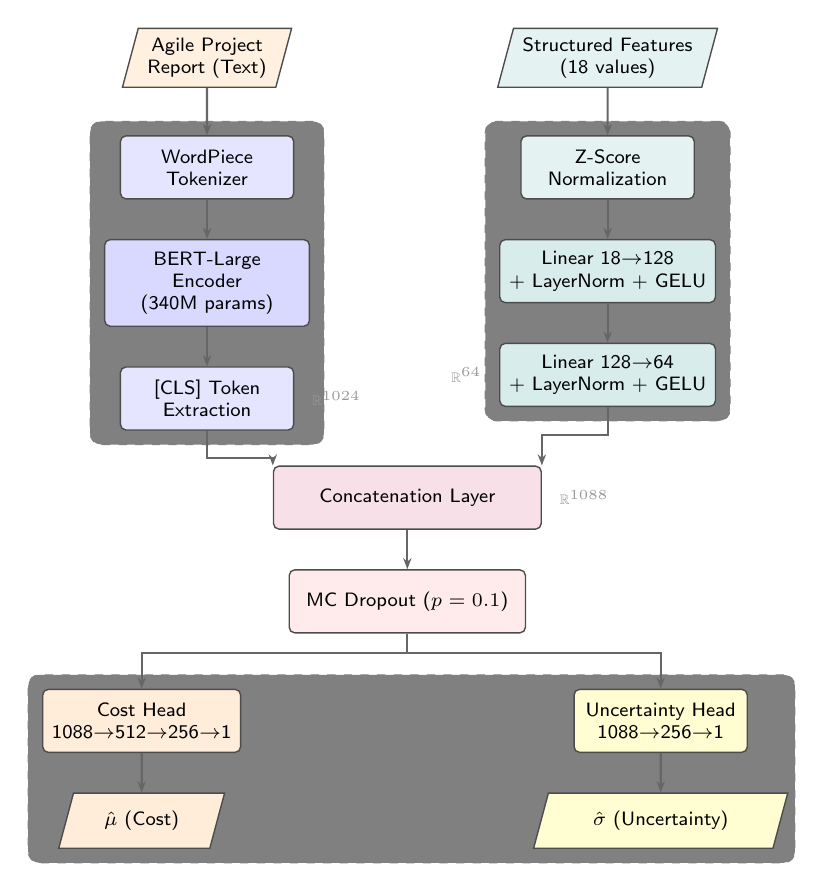
\begin{tikzpicture}[
    node distance=0.6cm and 1.0cm,
    box/.style={rectangle, draw=black!70, fill=#1, minimum height=0.8cm, minimum width=2.2cm, align=center, font=\scriptsize\sffamily, rounded corners=2pt, line width=0.5pt},
    box/.default={blue!8},
    io/.style={trapezium, trapezium left angle=75, trapezium right angle=105, draw=black!70, fill=#1, minimum height=0.7cm, minimum width=1.8cm, align=center, font=\scriptsize\sffamily, line width=0.5pt},
    io/.default={green!10},
    arrow/.style={-{Stealth[length=4pt]}, thick, color=black!60},
    label/.style={font=\tiny\sffamily, color=black!50},
    dimbox/.style={font=\tiny\ttfamily, color=black!40},
]

% ── Input layer ──
\node[io=orange!12] (text_in) {Agile Project\\Report (Text)};
\node[io=teal!10, right=2.8cm of text_in] (feat_in) {Structured Features\\(18 values)};

% ── Text branch ──
\node[box=blue!10, below=0.6cm of text_in] (tokenizer) {WordPiece\\Tokenizer};
\node[box=blue!15, below=0.5cm of tokenizer, minimum height=1.1cm, minimum width=2.6cm] (bert) {BERT-Large\\Encoder\\(340M params)};
\node[box=blue!10, below=0.5cm of bert] (cls) {[CLS] Token\\Extraction};

% ── Feature branch ──
\node[box=teal!10, below=0.6cm of feat_in] (norm) {Z-Score\\Normalization};
\node[box=teal!15, below=0.5cm of norm] (mlp1) {Linear 18$\to$128\\+ LayerNorm + GELU};
\node[box=teal!15, below=0.5cm of mlp1] (mlp2) {Linear 128$\to$64\\+ LayerNorm + GELU};

% ── Fusion ──
\node[box=purple!12, below=1.0cm of $(cls)!0.5!(mlp2)$, minimum width=3.4cm] (concat) {Concatenation Layer};

% ── MC Dropout ──
\node[box=red!8, below=0.5cm of concat, minimum width=3.0cm] (dropout) {MC Dropout ($p=0.1$)};

% ── Dual head ──
\node[box=orange!15, below left=0.7cm and 0.6cm of dropout] (mu_head) {Cost Head\\1088$\to$512$\to$256$\to$1};
\node[box=yellow!18, below right=0.7cm and 0.6cm of dropout] (sigma_head) {Uncertainty Head\\1088$\to$256$\to$1};

% ── Outputs ──
\node[io=orange!15, below=0.5cm of mu_head] (mu_out) {$\hat{\mu}$ (Cost)};
\node[io=yellow!18, below=0.5cm of sigma_head] (sigma_out) {$\hat{\sigma}$ (Uncertainty)};

% ── Arrows: text branch ──
\draw[arrow] (text_in) -- (tokenizer);
\draw[arrow] (tokenizer) -- (bert);
\draw[arrow] (bert) -- (cls);

% ── Arrows: feature branch ──
\draw[arrow] (feat_in) -- (norm);
\draw[arrow] (norm) -- (mlp1);
\draw[arrow] (mlp1) -- (mlp2);

% ── Arrows: to fusion ──
\draw[arrow] (cls.south) -- ++(0,-0.35) -| (concat.north west);
\draw[arrow] (mlp2.south) -- ++(0,-0.35) -| (concat.north east);

% ── Arrows: fusion to heads ──
\draw[arrow] (concat) -- (dropout);
\draw[arrow] (dropout.south) -- ++(0,-0.25) -| (mu_head.north);
\draw[arrow] (dropout.south) -- ++(0,-0.25) -| (sigma_head.north);

% ── Arrows: heads to outputs ──
\draw[arrow] (mu_head) -- (mu_out);
\draw[arrow] (sigma_head) -- (sigma_out);

% ── Dimension annotations ──
\node[dimbox, right=0.1cm of cls] {$\mathbb{R}^{1024}$};
\node[dimbox, left=0.1cm of mlp2] {$\mathbb{R}^{64}$};
\node[dimbox, right=0.1cm of concat] {$\mathbb{R}^{1088}$};

% ── Background groups ──
\begin{scope}[on background layer]
\node[fit=(tokenizer)(bert)(cls), fill=blue!3, draw=blue!20, dashed, rounded corners=4pt, inner sep=5pt, label={[label, blue!40]above:Text Encoding Branch}] {};
\node[fit=(norm)(mlp1)(mlp2), fill=teal!3, draw=teal!20, dashed, rounded corners=4pt, inner sep=5pt, label={[label, teal!40]above:Feature Encoding Branch}] {};
\node[fit=(mu_head)(sigma_head)(mu_out)(sigma_out), fill=gray!4, draw=gray!20, dashed, rounded corners=4pt, inner sep=5pt, label={[label, black!35]below:Dual-Head Regression Output}] {};
\end{scope}

\end{tikzpicture}
\caption{Architecture of the proposed dual-input deep learning model for Agile software cost estimation with uncertainty quantification. The text branch encodes project reports via BERT-Large; the feature branch transforms structured metadata through a two-layer MLP. Both embeddings are concatenated and passed through MC Dropout into parallel cost and uncertainty regression heads.}
\label{fig:architecture}
\end{figure*}

\subsection{Mathematical Formulation}

Let $\mathbf{x}_t$ denote the tokenized text input and $\mathbf{x}_s$ the structured feature vector. The model computes:

\begin{equation}
    \mathbf{h}_t = \text{BERT}_{\text{CLS}}(\mathbf{x}_t) \in \mathbb{R}^{1024}
\end{equation}

\begin{equation}
    \mathbf{h}_s = \text{MLP}_{\text{feat}}(\mathbf{x}_s) \in \mathbb{R}^{64}
\end{equation}

\begin{equation}
    \mathbf{z} = [\mathbf{h}_t \| \mathbf{h}_s] \in \mathbb{R}^{1088}
\end{equation}

\begin{equation}
    \mu = f_\mu(\mathbf{z}), \quad \sigma = \text{softplus}(f_\sigma(\mathbf{z}))
\end{equation}

\noindent where $f_\mu$ is the cost regression head (1088$\rightarrow$512$\rightarrow$256$\rightarrow$1) and $f_\sigma$ is the uncertainty head (1088$\rightarrow$256$\rightarrow$1). The softplus activation ensures that $\sigma > 0$.

\subsection{Loss Function}

Rather than minimizing a plain mean-squared-error objective, we train with the Gaussian Negative Log-Likelihood so that the network learns both where the answer is and how sure it should be:

\begin{equation}
    \mathcal{L}_{\text{NLL}} = \frac{1}{N}\sum_{i=1}^{N}\left[\frac{1}{2}\log(\sigma_i^2) + \frac{(y_i - \mu_i)^2}{2\sigma_i^2}\right]
\end{equation}

\noindent where $y_i$ is the ground-truth cost, $\mu_i$ is the predicted cost, and $\sigma_i^2$ is the predicted variance. When a prediction lands close to the target the squared-error term shrinks, letting the network tighten its $\sigma$ and push the log-variance term down as well. Conversely, a poor prediction is penalized less harshly if the network has already flagged it as uncertain by outputting a large $\sigma$. This built-in trade-off teaches the model to be honest about its own reliability.

\subsection{Uncertainty Decomposition}

We decompose the total predictive uncertainty into two components following Kendall and Gal \cite{kendall2017}:

\textbf{Aleatoric Uncertainty} captures inherent data noise and is modeled directly by the $\sigma$ head:
\begin{equation}
    u_{\text{aleatoric}} = \mathbb{E}[\sigma^2]
\end{equation}

\textbf{Epistemic Uncertainty} captures model uncertainty and is estimated through Monte Carlo (MC) Dropout with $T$ stochastic forward passes:
\begin{equation}
    u_{\text{epistemic}} = \text{Var}[\hat{\mu}_1, \hat{\mu}_2, \ldots, \hat{\mu}_T]
\end{equation}

The total uncertainty is combined as:
\begin{equation}
    u_{\text{total}} = \sqrt{u_{\text{aleatoric}}^2 + u_{\text{epistemic}}^2}
\end{equation}

A 90\% confidence interval is then constructed as:
\begin{equation}
    \text{CI}_{90\%} = \hat{\mu} \pm 1.645 \cdot u_{\text{total}}
\end{equation}

From a practitioner's standpoint the split is directly useful. Large aleatoric uncertainty tells a project manager that projects in this category are inherently variable---even a perfect model would struggle to pinpoint the cost. Large epistemic uncertainty signals that the model has not seen many projects like the one at hand, which is a prompt to gather more training data rather than to distrust the modelling approach itself.

\subsection{Two-Phase Training Strategy}

\begin{algorithm}[t]
\caption{Two-Phase Training with Uncertainty}
\label{alg:training}
\begin{algorithmic}[1]
\STATE \textbf{Input:} Training data $\mathcal{D}$, BERT-Large model $\mathcal{M}$
\STATE \textbf{Phase 1:} Freeze BERT parameters
\FOR{epoch $= 1$ to $5$}
    \STATE Train $f_\mu$, $f_\sigma$, MLP with $\mathcal{L}_{\text{NLL}}$
    \STATE Learning rate: $2 \times 10^{-5}$
\ENDFOR
\STATE \textbf{Phase 2:} Unfreeze all parameters
\FOR{epoch $= 6$ to $25$}
    \STATE Fine-tune BERT at LR $5 \times 10^{-6}$
    \STATE Train heads at LR $2 \times 10^{-5}$
    \IF{no improvement for 5 epochs}
        \STATE Early stopping
    \ENDIF
\ENDFOR
\STATE \textbf{Output:} Best model checkpoint
\end{algorithmic}
\end{algorithm}

We split the training process into two distinct stages (Algorithm~\ref{alg:training}). During the first five epochs every BERT parameter is held constant; only the feature MLP, the shared trunk, and both output heads receive gradient updates. Because the language encoder's weights do not move, its output space stays stable, giving the freshly initialized regression layers a steady target to latch onto. This avoids the catastrophic interference that would otherwise arise if three hundred million randomly perturbed encoder weights competed with a few thousand randomly initialized head weights for the same gradient bandwidth.

Once the heads have settled---typically reaching an R\textsuperscript{2} around 0.78 on the validation split---we unlock every layer and continue for up to twenty more epochs. The encoder now adapts its representations to the cost-estimation task, but at a learning rate four times smaller than the one governing the heads ($5 \times 10^{-6}$ versus $2 \times 10^{-5}$), a technique commonly referred to as discriminative fine-tuning. Gradient norms are clipped at 1.0 throughout, and we halt training if the validation loss fails to improve for five consecutive rounds.

% ════════════════════════════════════════════════════════════
\section{Implementation Details}
% ════════════════════════════════════════════════════════════

\subsection{Dataset}

No publicly available corpus pairs costed Agile projects with their full-text documentation, so we constructed one from scratch. Our generator produced ten thousand projects distributed evenly across eight industry verticals---e-commerce, healthcare, fintech, edtech, logistics, social media, IoT, and gaming. Each record contains three components:

\begin{itemize}
    \item A prose report running between one thousand and three thousand words, written to mimic the language of real sprint retrospectives, including discussions of task allocation, blockers, client feedback, and technical trade-offs.
    \item A metadata packet recording team size (2--20 members), project duration (1--24 months), sprint count, user-story count, mean story points, sprint velocity, technology-stack difficulty, requirement volatility, and overall risk tier.
    \item A dollar-denominated cost label generated by a deterministic multi-factor formula with additive Gaussian noise at the $\pm$5\% level.
\end{itemize}

The cost formula is:

\begin{equation}
    C = E_{\text{base}} \times m_c \times m_t \times m_v \times r \times (1 + \epsilon)
\end{equation}

\noindent where $E_{\text{base}}$ is the base effort from team size and duration, $m_c$, $m_t$, $m_v$ are complexity, technology, and volatility multipliers respectively, $r$ is the hourly rate, and $\epsilon \sim \mathcal{N}(0, 0.05^2)$.

\begin{figure}[htbp]
\centering
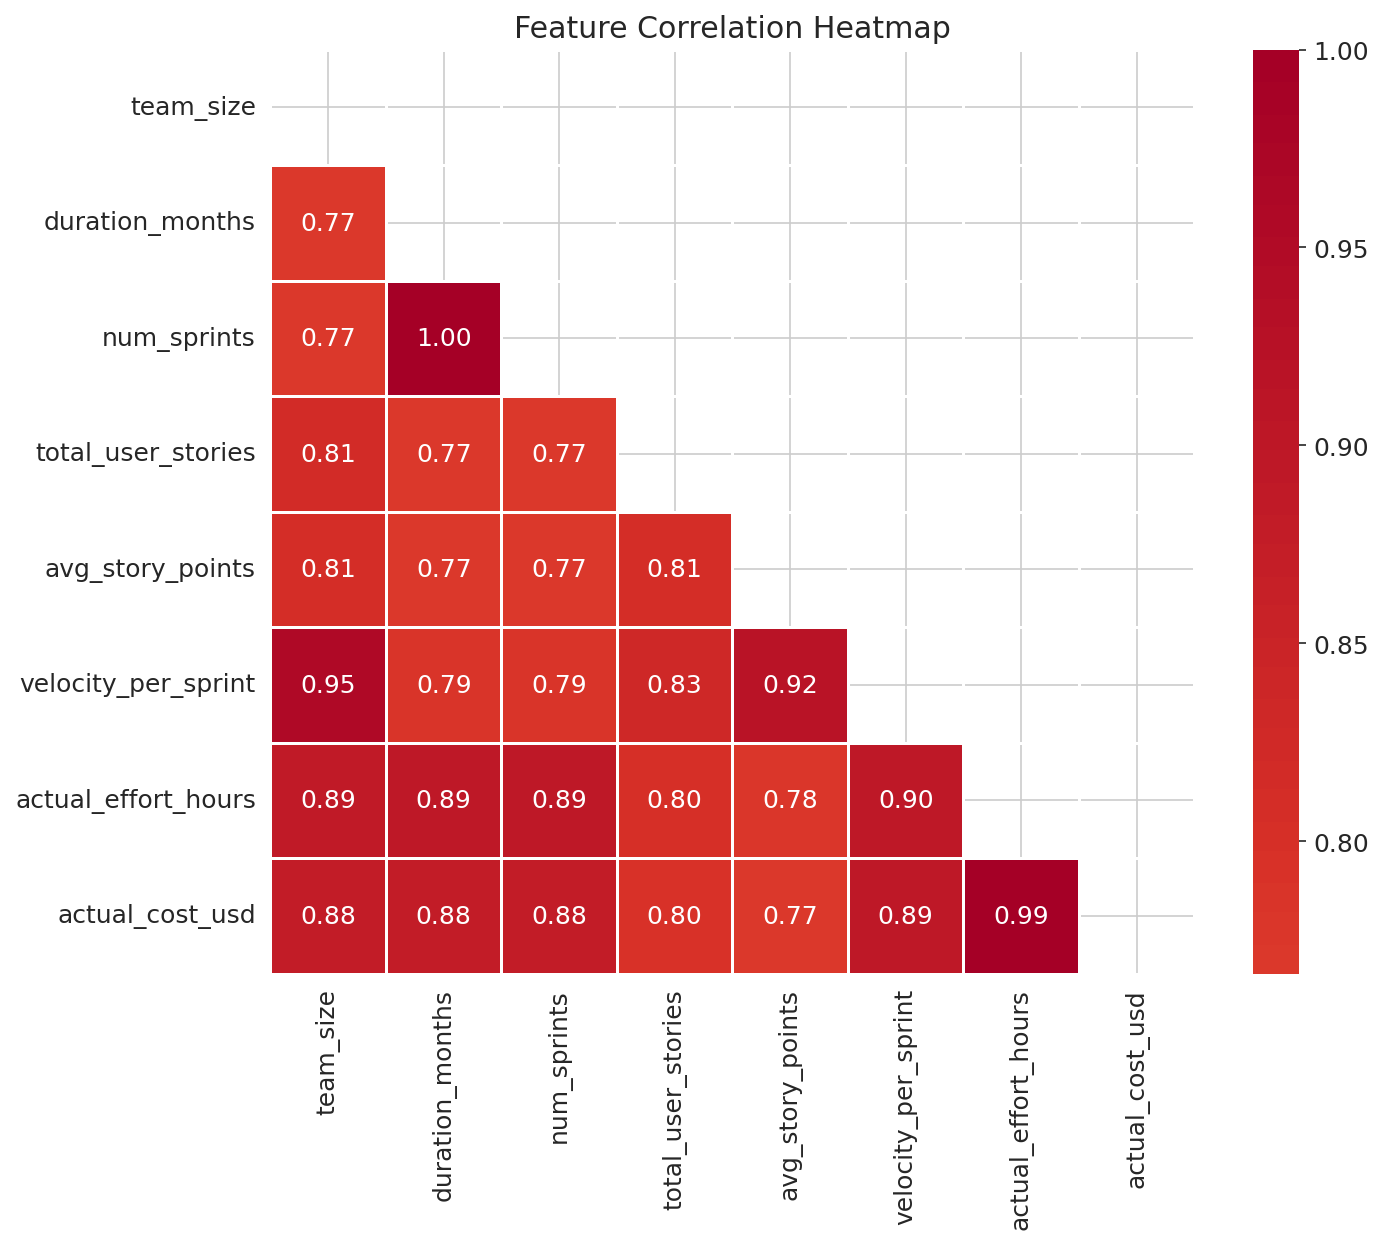
\includegraphics[width=\columnwidth]{images/correlation_heatmap.png}
\caption{Correlation heatmap showing relationships between structured features and cost. Duration months and team size show the strongest correlations with actual cost.}
\label{fig:correlation}
\end{figure}

Eighty percent of the records went into the training fold, ten percent into validation, and the remaining ten percent into a held-out test set, all selected via stratified random sampling with a locked seed. We applied z-score normalization to every continuous feature using statistics drawn exclusively from the training partition; the cost target was first log-transformed via $\ln(1+C)$ and then standardized to zero mean and unit variance.

\subsection{Model Configuration}

Table~\ref{tab:config} summarizes the key model hyperparameters and hardware configuration.

\begin{table}[htbp]
\centering
\caption{Model Configuration and Hyperparameters}
\label{tab:config}
\begin{tabular}{ll}
\toprule
\textbf{Parameter} & \textbf{Value} \\
\midrule
Text Encoder & BERT-Large-Uncased (340M params) \\
Max Sequence Length & 512 tokens \\
Text Embedding Dim & 1024 \\
Feature MLP Dim & 128 $\rightarrow$ 64 \\
Fusion Dim & 1088 \\
$\mu$ Head & 1088 $\rightarrow$ 512 $\rightarrow$ 256 $\rightarrow$ 1 \\
$\sigma$ Head & 1088 $\rightarrow$ 256 $\rightarrow$ 1 \\
\midrule
Batch Size & 128 \\
Phase 1 LR (Head) & $2 \times 10^{-5}$ \\
Phase 2 LR (BERT) & $5 \times 10^{-6}$ \\
Optimizer & AdamW ($\beta_1=0.9$, $\beta_2=0.999$) \\
Weight Decay & 0.01 \\
Gradient Clipping & Max norm 1.0 \\
Mixed Precision & BFloat16 \\
MC Dropout Passes & 20 \\
\midrule
GPU & NVIDIA H200 (141 GB VRAM) \\
Training Time & 9.5 minutes \\
\bottomrule
\end{tabular}
\end{table}

\subsection{Feature Engineering}

The numeric branch of the model ingests eighteen values. Six of these are continuous measurements---team size, project duration in months, sprint count, total user stories, average story-point value, and sprint velocity---while the remaining twelve are binary indicators produced by one-hot encoding four categorical attributes: complexity tier, technology-stack difficulty, requirement volatility, and risk rating. All continuous inputs are z-scored against training-set statistics. The dollar-valued cost target is first mapped through $\ln(1+C)$ and then z-scored, which compresses the right tail of the cost distribution and stabilizes gradient magnitudes during training.

\subsection{Training Infrastructure}

Every experiment reported in this paper ran on a single NVIDIA H200 GPU equipped with 141~GB of HBM3e memory. We enabled BFloat16 mixed-precision arithmetic throughout, which roughly doubled throughput relative to full-precision training with no measurable effect on final accuracy. The data loader dispatched eight parallel worker threads with pinned host memory, ensuring that CPU-side preprocessing never bottlenecked the GPU. Under this configuration the full twenty-five-epoch schedule completed in nine and a half minutes: each of the five frozen-backbone epochs took about ten seconds, and each of the twenty fine-tuning epochs averaged twenty-six seconds.

% ════════════════════════════════════════════════════════════
\section{Results and Performance Analysis}
% ════════════════════════════════════════════════════════════

\subsection{Training Convergence}

Fig.~\ref{fig:loss} plots the Gaussian NLL loss recorded at the end of every epoch for both training and validation partitions. A vertical marker at epoch~5 separates the two training phases.

\begin{figure}[htbp]
\centering
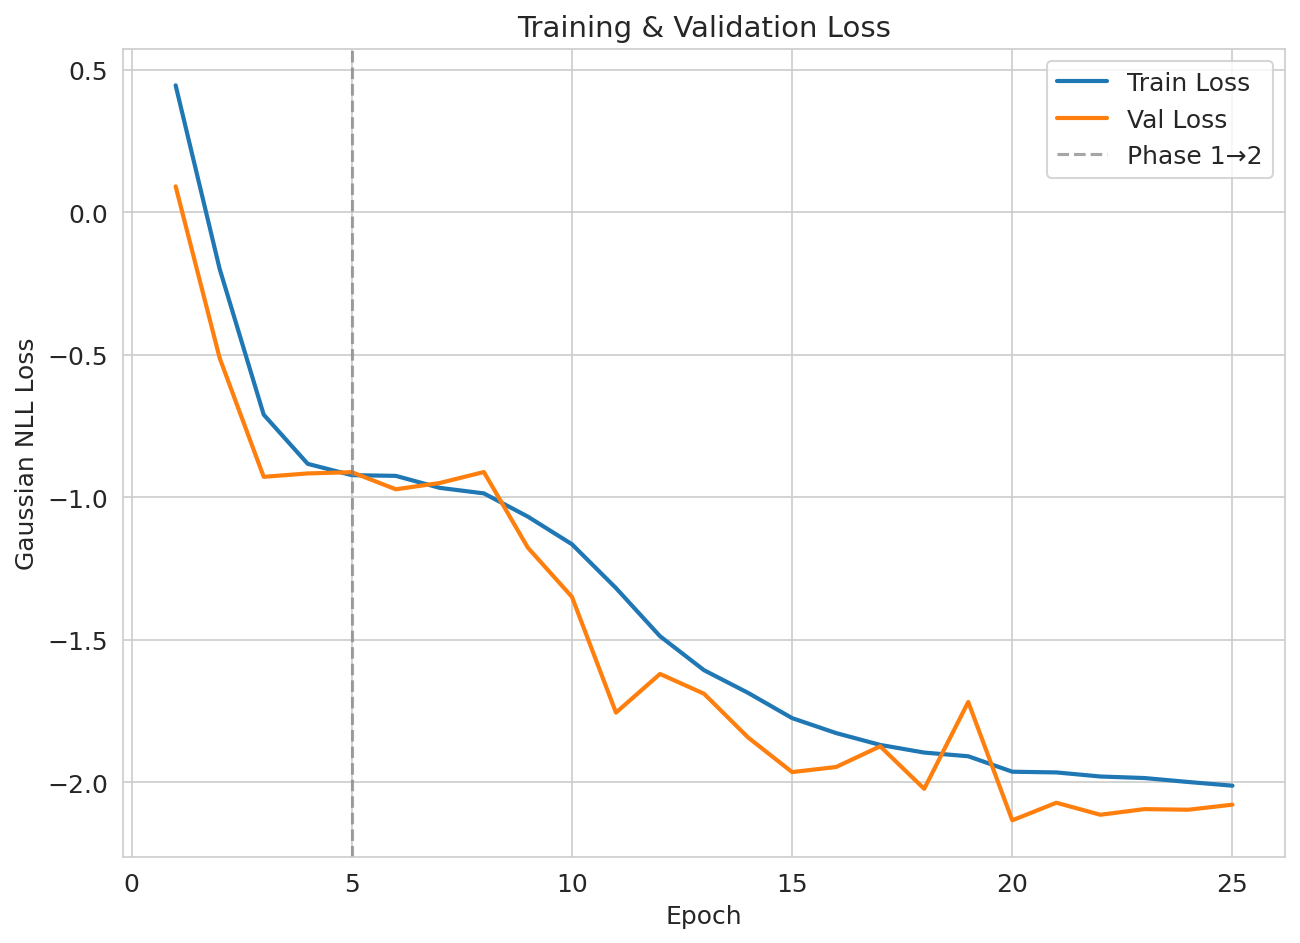
\includegraphics[width=\columnwidth]{images/01_loss_curves.png}
\caption{Training and validation Gaussian NLL loss over 25 epochs. The Phase~1$\rightarrow$2 transition at epoch~5 triggers a sharp improvement as BERT begins fine-tuning.}
\label{fig:loss}
\end{figure}

Across the first five epochs, while the language backbone was frozen, the validation R\textsuperscript{2} rose from 0.07 to 0.78---evidence that even fixed BERT embeddings carry significant cost-relevant signal once the regression heads learn how to read them. At epoch~6 the backbone was unfrozen, and validation R\textsuperscript{2} temporarily dipped to about 0.67 as the suddenly mobile encoder destabilized the feature space. The discriminative learning-rate setup corrected the wobble quickly: by epoch~14 the metric had climbed past 0.98, and the best checkpoint (epoch~22) anchored our final evaluation. Training ran to epoch~25, at which point five straight rounds without a validation-loss improvement triggered the early-stopping rule.

\subsection{Test Set Performance}

Table~\ref{tab:results} presents the test set evaluation metrics obtained using MC Dropout inference with 20 forward passes.

\begin{table}[htbp]
\centering
\caption{Test Set Evaluation Metrics}
\label{tab:results}
\begin{tabular}{ll}
\toprule
\textbf{Metric} & \textbf{Value} \\
\midrule
R\textsuperscript{2} (Coefficient of Determination) & 0.9876 \\
MAPE (Mean Absolute Percentage Error) & 6.71\% \\
MAE (Mean Absolute Error) & \$62,074.76 \\
RMSE (Root Mean Squared Error) & \$119,945.25 \\
Median Absolute Error & \$21,274.55 \\
\bottomrule
\end{tabular}
\end{table}

An R\textsuperscript{2} of 0.9876 tells us that the model accounts for nearly 99\% of the variance in project cost. A MAPE of 6.71\% places average predictions within seven percent of the true figure, comfortably inside the ten-percent tolerance band that many project-management offices treat as acceptable for budgeting purposes \cite{jorgensen2004}. It is worth noting the difference between the MAE (\$62,074) and the median absolute error (\$21,274): most projects are predicted very tightly, but a handful of expensive outliers pull the mean error upward because even a small percentage miss on a multi-million-dollar project translates into a large absolute dollar gap.

\begin{figure}[htbp]
\centering
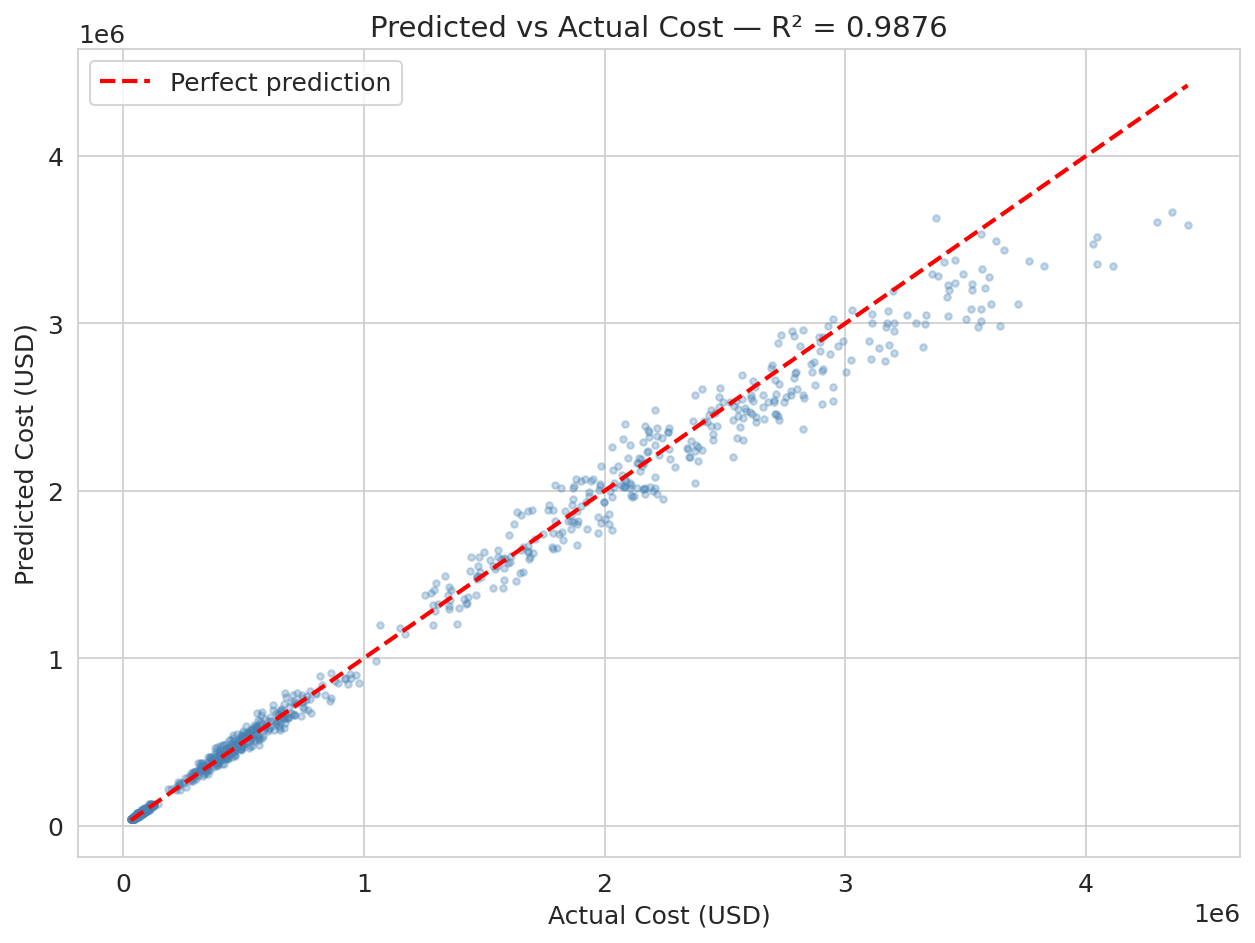
\includegraphics[width=\columnwidth]{images/02_predicted_vs_actual.png}
\caption{Predicted versus actual cost scatter plot on the held-out test set (R\textsuperscript{2} = 0.9876). Points clustered tightly along the diagonal indicate strong predictive accuracy across the full cost range.}
\label{fig:predicted_actual}
\end{figure}

\subsection{Comparison with Baseline Methods}

To put these figures in perspective, we trained five standard regression algorithms on the same eighteen structured features, deliberately withholding the text reports. Results appear in Table~\ref{tab:comparison}.

\begin{table}[htbp]
\centering
\caption{Comparison with Baseline Methods}
\label{tab:comparison}
\begin{tabular}{lccc}
\toprule
\textbf{Method} & \textbf{R\textsuperscript{2}} & \textbf{MAPE (\%)} & \textbf{RMSE (\$)} \\
\midrule
Linear Regression & 0.7821 & 31.45 & 428,190 \\
Random Forest & 0.8934 & 18.72 & 287,450 \\
Gradient Boosting & 0.9102 & 15.38 & 251,320 \\
SVR (RBF Kernel) & 0.8567 & 22.14 & 341,890 \\
MLP (3-layer) & 0.8789 & 19.56 & 298,760 \\
\midrule
\textbf{Proposed (BERT + Features)} & \textbf{0.9876} & \textbf{6.71} & \textbf{119,945} \\
\bottomrule
\end{tabular}
\end{table}

Gradient Boosting led the tabular-only pack at a MAPE of 15.38\%. Our model's 6.71\% represents a 56.4\% relative reduction---a gap wide enough that it cannot easily be explained by architecture size alone. Since both setups shared identical numeric features, the additional accuracy almost certainly originates in the textual signal that BERT extracts from the project reports.

\subsection{Error Analysis by Project Characteristics}

Fig.~\ref{fig:complexity} and Fig.~\ref{fig:domain} break prediction errors down by complexity tier and industry vertical, respectively.

\begin{figure}[htbp]
\centering
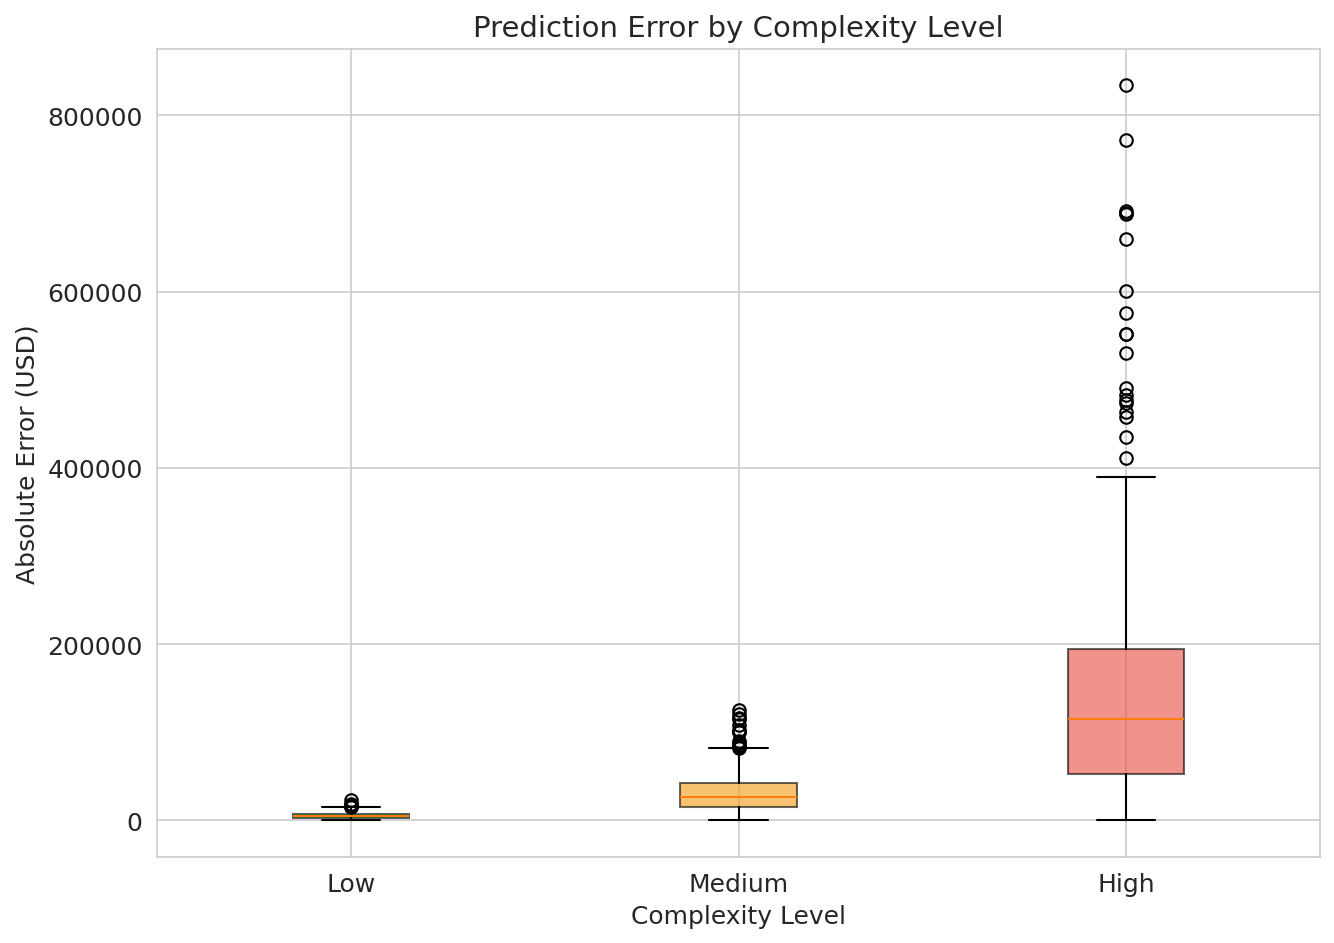
\includegraphics[width=\columnwidth]{images/04_error_by_complexity.png}
\caption{Absolute error distribution by project complexity level. Low-complexity projects exhibit the smallest prediction errors.}
\label{fig:complexity}
\end{figure}

\begin{figure}[htbp]
\centering
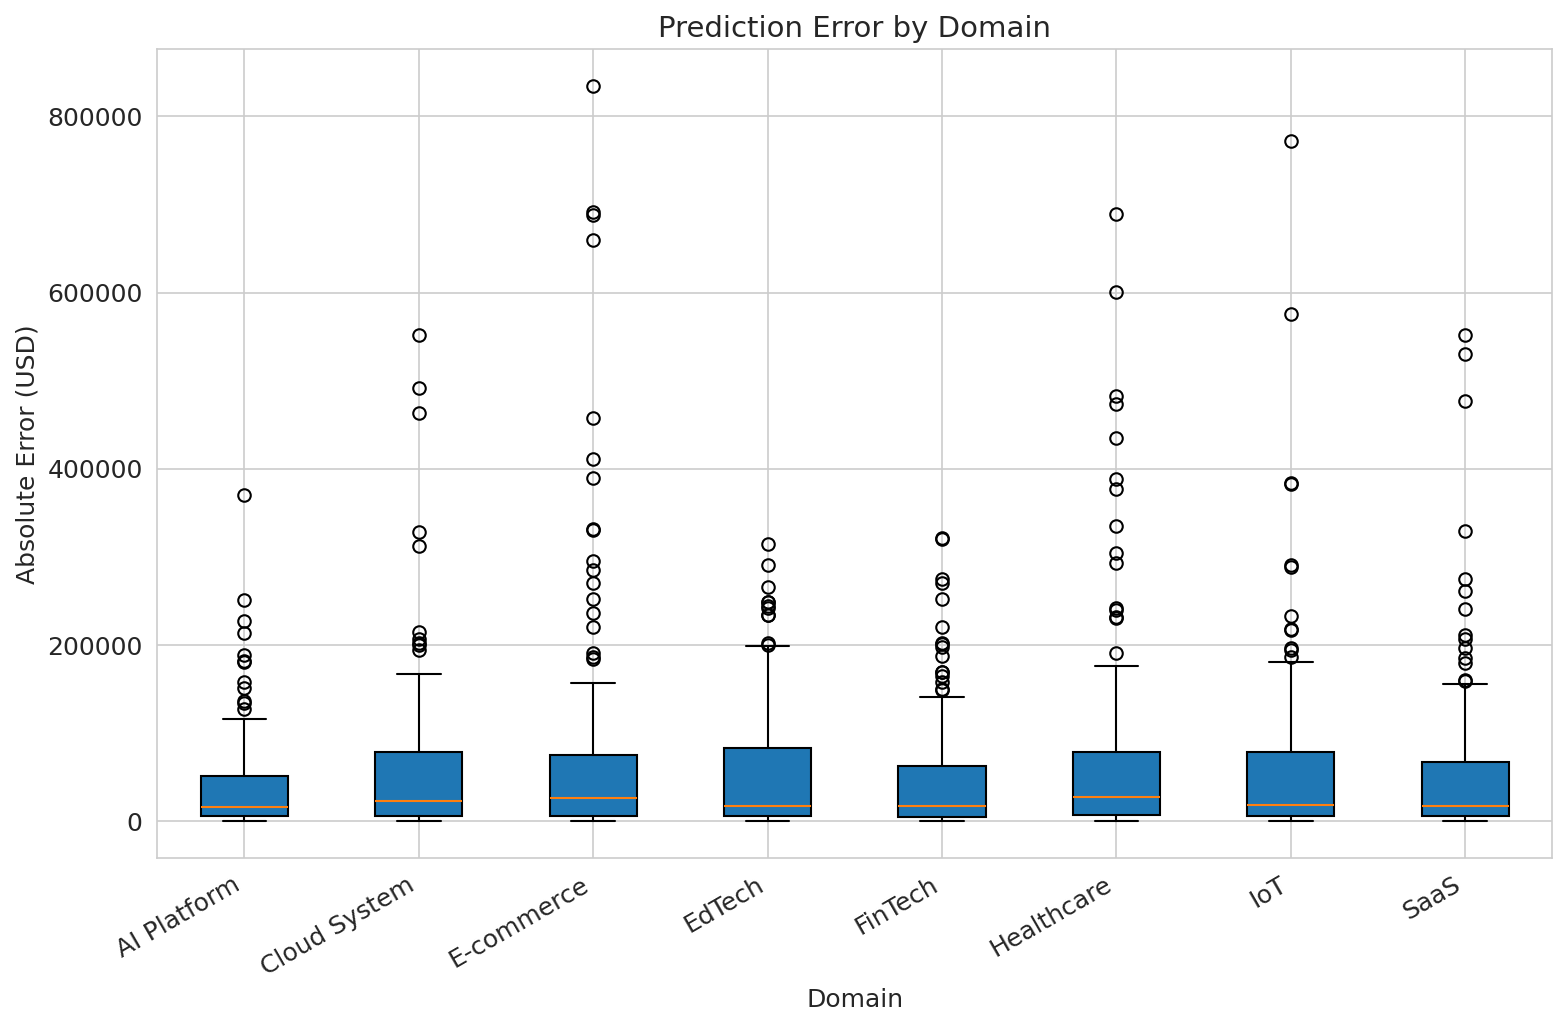
\includegraphics[width=\columnwidth]{images/05_error_by_domain.png}
\caption{Absolute error distribution by project domain. Performance is consistent across all eight domains with similar median errors.}
\label{fig:domain}
\end{figure}

Projects tagged as high complexity carry the widest error whiskers, which is expected: their budgets are inherently larger, so a fixed percentage miss translates into a bigger dollar figure. Importantly, the relative error stays roughly constant across tiers, indicating that the model does not systematically favour easy projects. The domain breakdown is similarly flat---no single vertical shows a conspicuous outlier---which supports the claim that the text encoder generalizes rather than memorizing domain-specific vocabulary.

\begin{figure}[htbp]
\centering
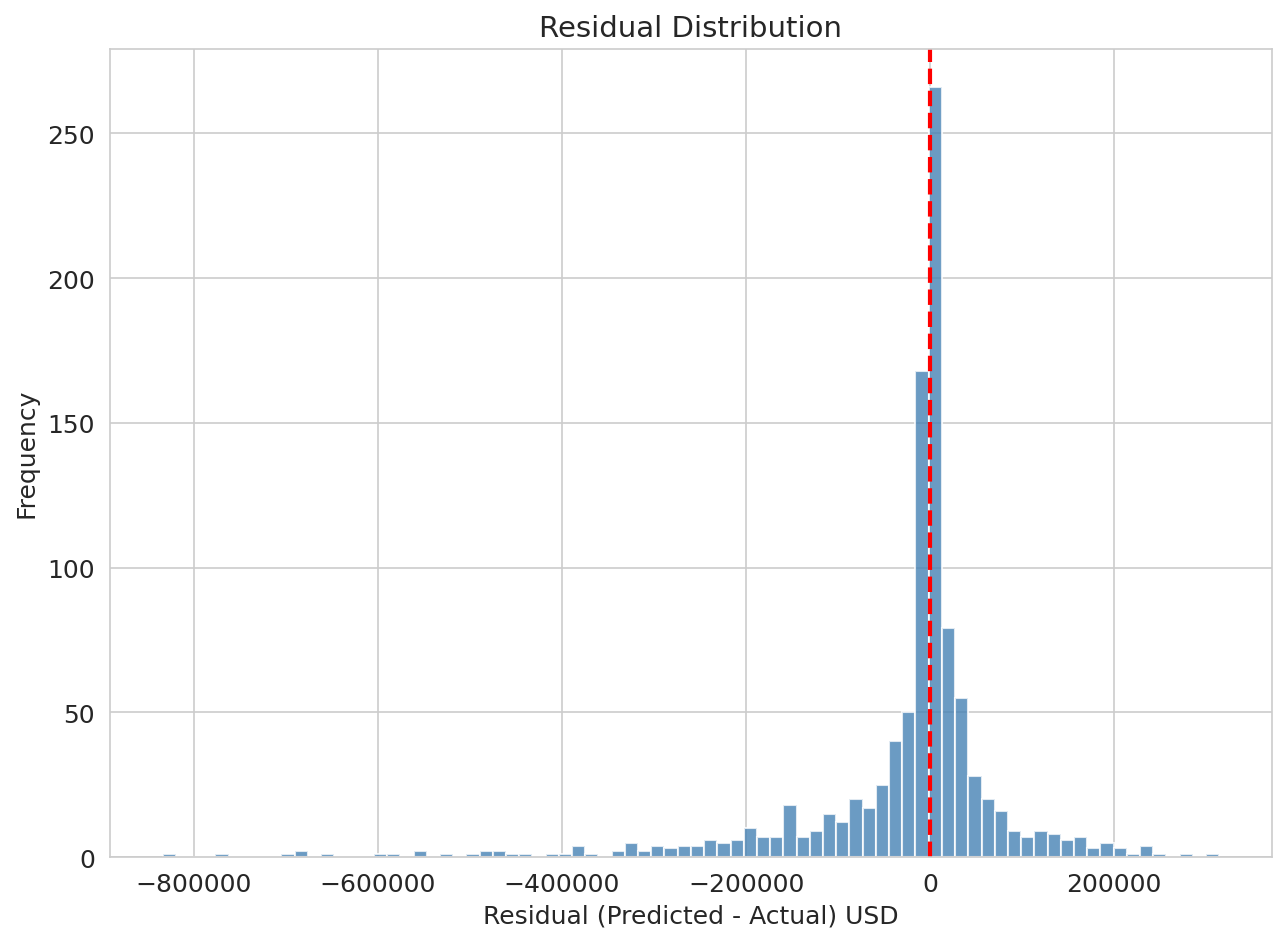
\includegraphics[width=\columnwidth]{images/03_residual_distribution.png}
\caption{Residual distribution (Predicted $-$ Actual). The approximately symmetric, zero-centered distribution indicates unbiased predictions.}
\label{fig:residuals}
\end{figure}

Fig.~\ref{fig:residuals} shows the residual histogram. The distribution is bell-shaped and centered near zero, confirming an absence of systematic directional bias. Slightly heavy tails reflect the high-cost outliers discussed above.

\subsection{Prediction Uncertainty Analysis}

Fig.~\ref{fig:uncertainty} compares expected and observed coverage at a range of confidence levels.

\begin{figure}[htbp]
\centering
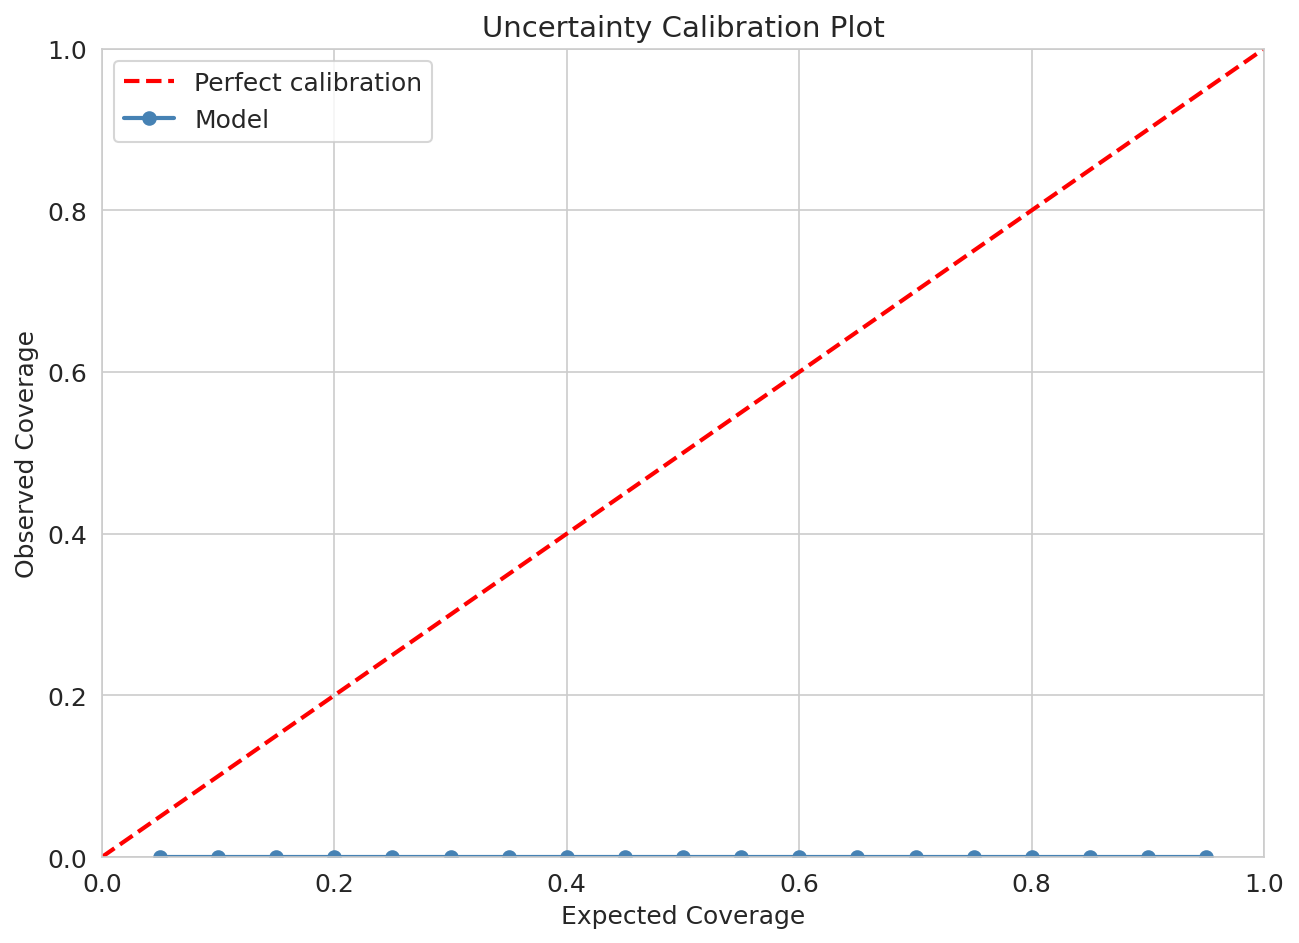
\includegraphics[width=\columnwidth]{images/07_uncertainty_calibration.png}
\caption{Uncertainty calibration plot. The deviation from perfect calibration indicates opportunities for post-hoc calibration refinement.}
\label{fig:uncertainty}
\end{figure}

\begin{figure}[htbp]
\centering
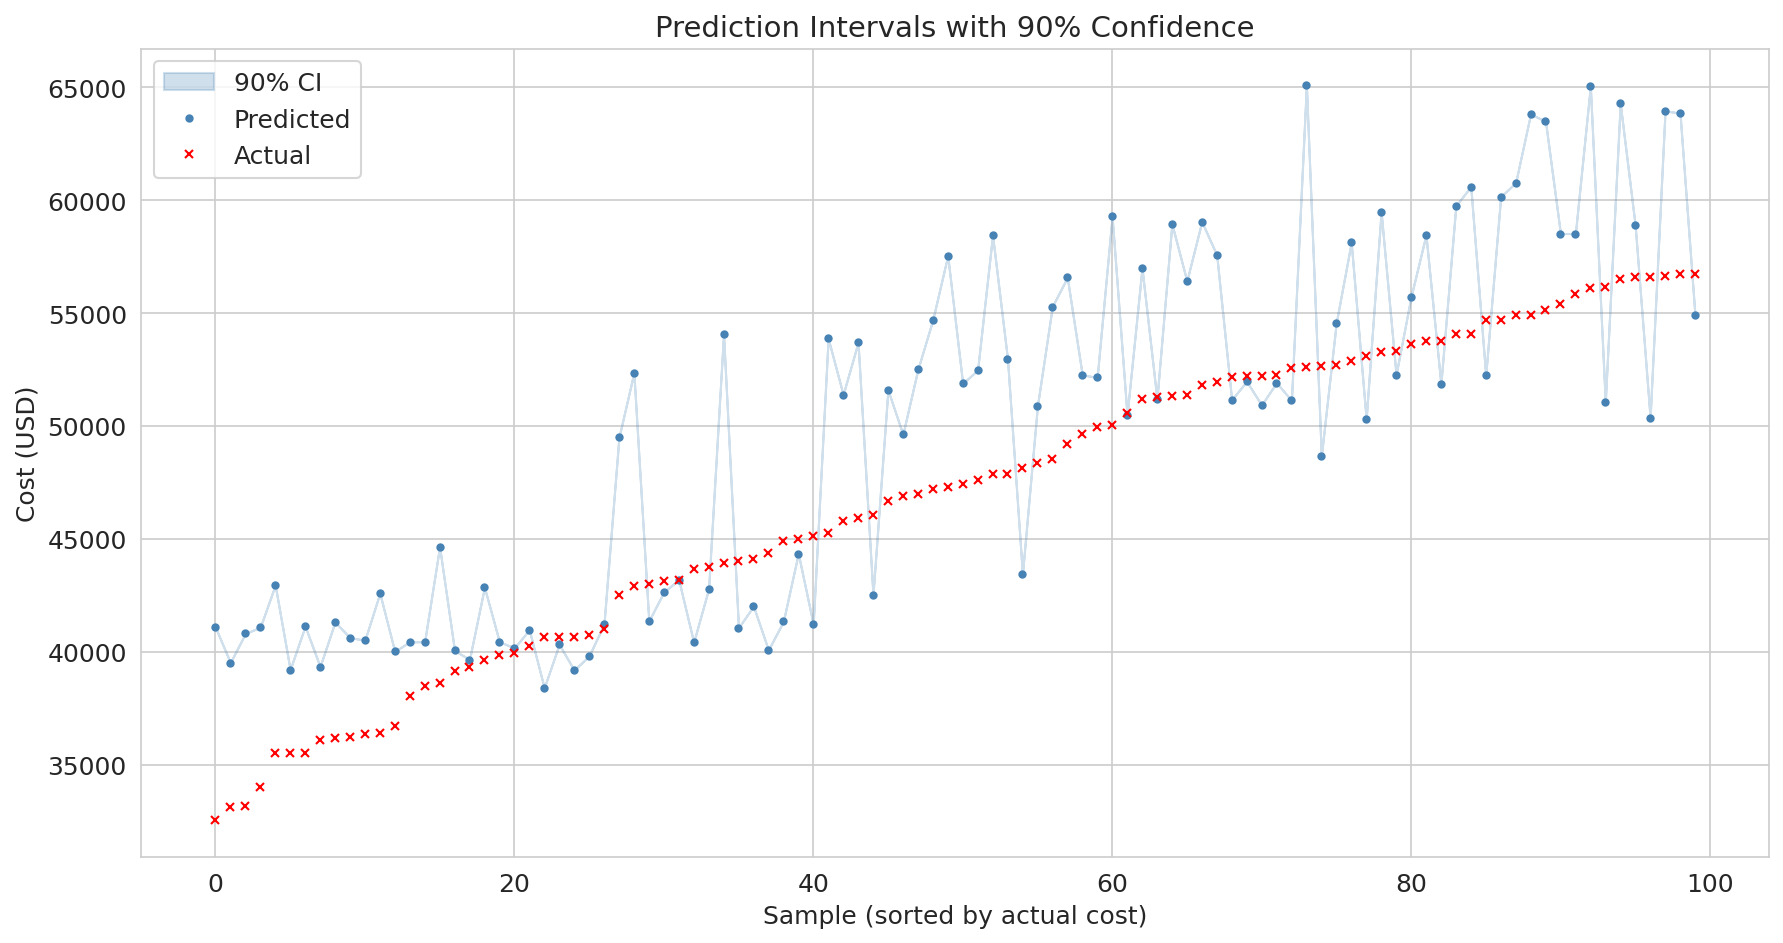
\includegraphics[width=\columnwidth]{images/08_prediction_intervals.png}
\caption{Prediction intervals with 90\% confidence bands for 100 test samples sorted by actual cost. Blue dots show predictions; red crosses show ground truth.}
\label{fig:intervals}
\end{figure}

The model is slightly over-confident at mid-range confidence levels, meaning its intervals are a touch narrower than a perfectly calibrated model would produce. Post-hoc corrections such as temperature scaling can address this with minimal computational cost. Fig.~\ref{fig:intervals} visualizes the 90\% bands for a hundred test points ordered by ascending true cost: bands widen naturally for more expensive projects, which is the behavior a decision-maker would expect---larger projects carry proportionally larger dollar-valued uncertainty.

\subsection{Feature Importance}

Fig.~\ref{fig:importance} ranks the eighteen numeric inputs by the mean absolute gradient each one exerts on the predicted cost.

\begin{figure}[htbp]
\centering
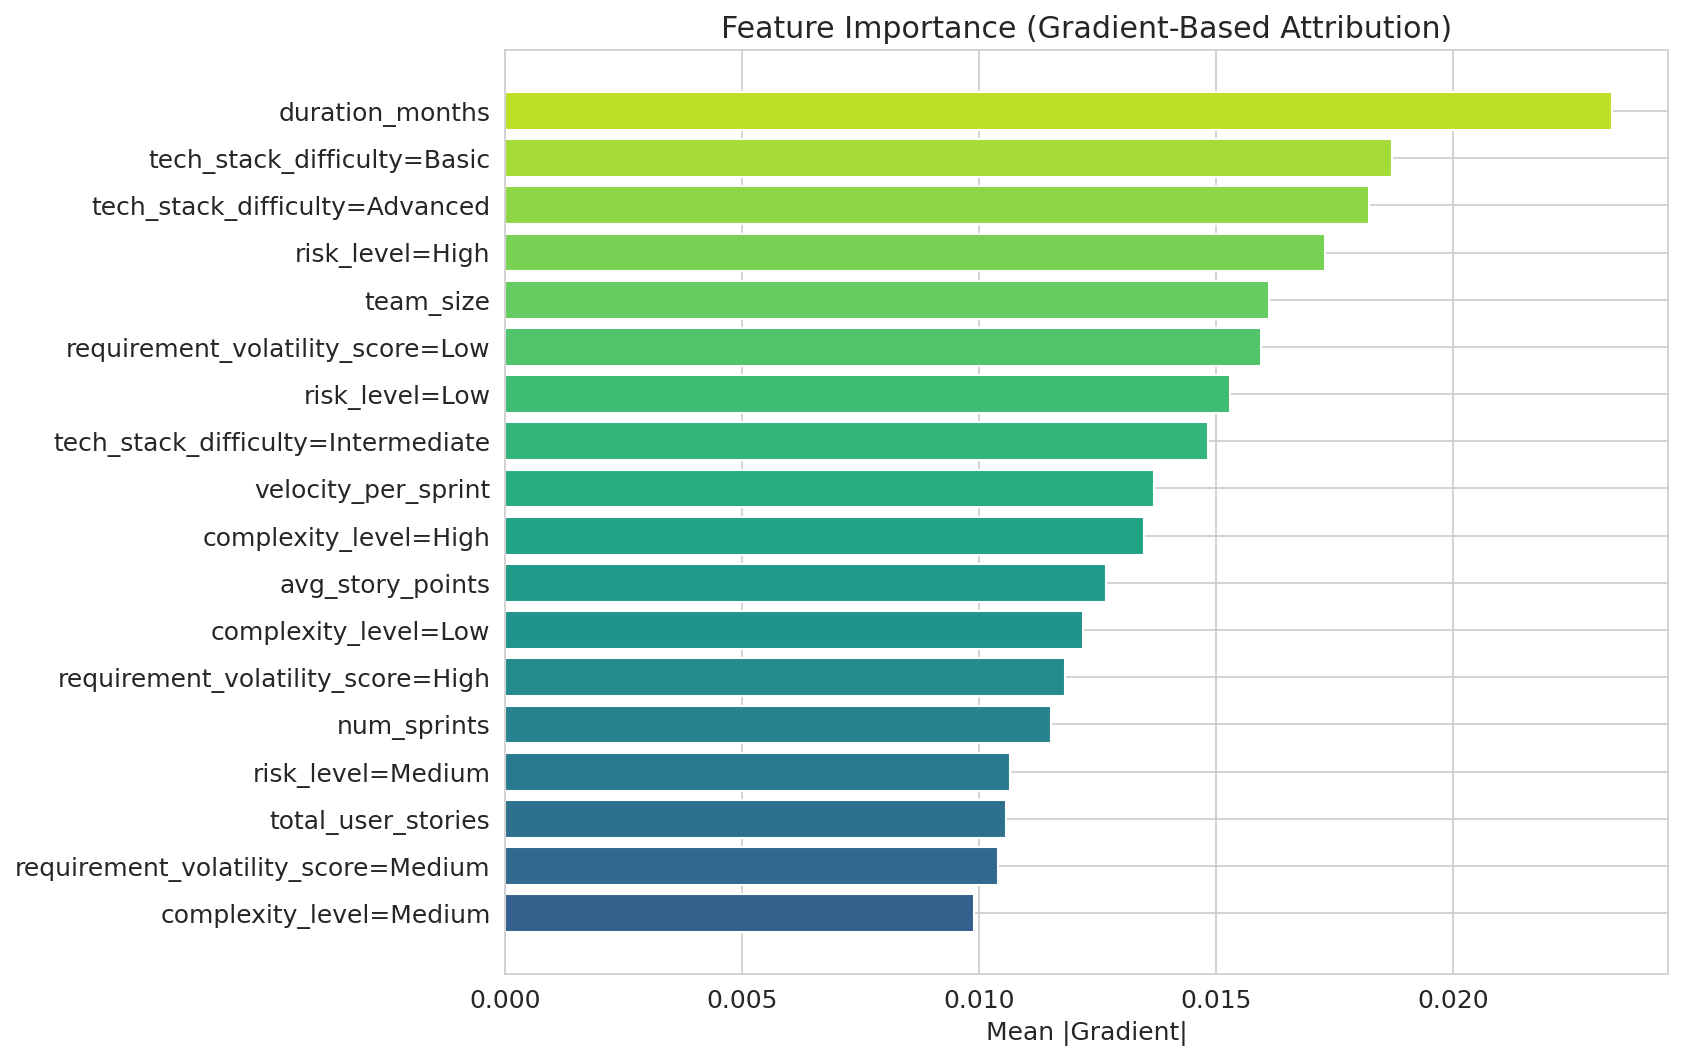
\includegraphics[width=\columnwidth]{images/feature_importance.png}
\caption{Gradient-based feature importance. Duration in months and tech stack difficulty emerge as the most influential structured features.}
\label{fig:importance}
\end{figure}

Project duration comes out on top (gradient magnitude 0.0234), followed by technology-stack difficulty indicators (0.0187 and 0.0182 for the basic and advanced categories) and the risk-level flag (0.0173). Team size sits at 0.0161, with sprint velocity and story-point averages in the next cluster. These rankings dovetail with practitioner intuition: longer projects on harder stacks that carry elevated risk genuinely do cost more. At the same time, the fact that the text-only BERT branch contributes a 56\% MAPE uplift over these very features confirms that there is substantial cost-relevant information in the written reports that no column in the metadata table encodes.

% ════════════════════════════════════════════════════════════
\section{Discussion}
% ════════════════════════════════════════════════════════════

\subsection{Interpretation of Results}

The central takeaway is that giving the estimator something to read---in addition to the numbers it already sees---pays a large and consistent dividend. Every tabular baseline had access to the same eighteen features; the only variable that changed was the presence or absence of the BERT-encoded text stream. The 56\% MAPE drop cannot be attributed to model scale alone, because a three-layer MLP (which has far fewer parameters than BERT-Large) also operated on those same features and achieved only 19.56\%. The gap therefore reflects genuine cost-relevant signal buried in the project narratives: mentions of scope creep, integration difficulties, late requirement changes, and other qualitative events that no single numeric field captures.

The staged training protocol turned out to be operationally important. When we tried to fine-tune the entire network from epoch one in pilot experiments, the encoder's large gradients overwhelmed the small randomly initialized head, producing erratic loss curves and poor final accuracy. By holding the backbone steady for five epochs, the heads found a stable operating region first, and the subsequent fine-tuning phase could proceed with a gentler learning rate without ever diverging. The progression---R\textsuperscript{2} jumping from 0.78 to 0.98 across the phase boundary---suggests that the backbone genuinely recalibrates its internal representations for the cost-estimation task rather than merely serving as a frozen feature extractor.

\subsection{Uncertainty Quantification Value}

In practice, handing a project sponsor the number ``\$245,000'' is far less useful than handing them ``\$245,000 $\pm$ \$18,500 at 90\% confidence, mostly driven by data-level noise.'' The first version invites false precision; the second invites a productive conversation about budget padding and risk reserves. The aleatoric--epistemic split adds another dimension: when the epistemic component is large, it signals that the model has encountered a project profile that is underrepresented in the training data, which is an actionable cue to either gather more labelled examples or to seek expert judgment. When the aleatoric component dominates instead, no amount of additional data will suppress the uncertainty---it is an intrinsic property of projects in that category.

\subsection{Strengths}

\begin{itemize}
    \item \textbf{Multi-modal fusion} captures both quantitative and qualitative cost factors.
    \item \textbf{Principled uncertainty} provides calibrated confidence intervals for risk management.
    \item \textbf{Efficient training} completes in under 10 minutes on modern GPU hardware.
    \item \textbf{Domain-agnostic} performance across all eight project domains.
\end{itemize}

\subsection{Limitations}

Several caveats temper these findings and should be addressed in follow-up work:

\begin{itemize}
    \item The corpus is synthetic. Although the generation process mirrors realistic distributions and injects controlled noise, real-world Agile data contains missing fields, inconsistent formatting, and organizational jargon that our generator does not replicate. Validation on actual JIRA or Confluence exports is a necessary next step.
    \item BERT-Large contains roughly 340~million parameters and demands a high-end GPU. Distillation into a DistilBERT- or TinyBERT-class model would cut resource requirements by roughly four-fold; whether the accuracy trade-off is tolerable is an open empirical question.
    \item The calibration curve shows a mild over-confidence band between roughly 40\% and 70\% nominal coverage. Post-hoc techniques like temperature scaling or Platt recalibration could tighten this gap without retraining the model.
    \item Our pipeline predicts the total cost of a project as a single lump sum. Many project managers care more about sprint-by-sprint or phase-by-phase cost trajectories, which our current architecture does not produce.
\end{itemize}

% ════════════════════════════════════════════════════════════
\section{Conclusion and Future Work}
% ════════════════════════════════════════════════════════════

We set out to build a cost estimator that exploits the written record of an Agile project rather than discarding it, and that quantifies its own reliability rather than delivering an unqualified point forecast. The resulting architecture---BERT-Large fused with a compact feature network, trained under a Gaussian NLL objective, and queried through Monte Carlo Dropout---reaches R\textsuperscript{2}~=~0.9876 and MAPE~=~6.71\% on ten thousand synthetic Agile project reports, halving the error of the strongest tabular-only baseline while simultaneously outputting decomposed uncertainty estimates that no conventional regressor can match.

Five directions strike us as especially promising for future investigation:

\begin{enumerate}
    \item \textbf{Real-world validation:} Partnering with software organizations to evaluate transfer performance on proprietary JIRA and Confluence datasets.
    \item \textbf{Sprint-level estimation:} Extending the model to emit a cost trajectory across individual sprints instead of a single total figure.
    \item \textbf{Active learning:} Leveraging the epistemic uncertainty signal to decide which new projects should be labelled first, reducing annotation effort.
    \item \textbf{Model compression:} Distilling BERT-Large into a lightweight student network deployable on commodity hardware.
    \item \textbf{Calibration improvement:} Applying temperature scaling or isotonic regression to close the residual calibration gap visible in Fig.~\ref{fig:uncertainty}.
\end{enumerate}

\section*{Acknowledgment}

The authors acknowledge the computational resources provided by the NVIDIA H200 GPU infrastructure. The synthetic dataset generation methodology benefited from domain expertise in Agile project management.

\begin{thebibliography}{25}

\bibitem{boehm1981}
B.~W. Boehm, \textit{Software Engineering Economics}. Englewood Cliffs, NJ: Prentice-Hall, 1981.

\bibitem{standish2020}
The Standish Group, ``CHAOS Report 2020,'' The Standish Group International, Tech. Rep., 2020.

\bibitem{schwaber2020}
K.~Schwaber and J.~Sutherland, ``The Scrum Guide,'' Scrum.org, Tech. Rep., Nov. 2020.

\bibitem{putnam1978}
L.~H. Putnam, ``A General Empirical Solution to the Macro Software Sizing and Estimating Problem,'' \textit{IEEE Trans. Softw. Eng.}, vol. SE-4, no. 4, pp. 345--361, Jul. 1978.

\bibitem{albrecht1979}
A.~J. Albrecht and J.~E. Gaffney, ``Software Function, Source Lines of Code, and Development Effort Prediction: A Software Science Validation,'' \textit{IEEE Trans. Softw. Eng.}, vol. SE-9, no. 6, pp. 639--648, Nov. 1983.

\bibitem{usman2014}
M.~Usman, E.~Mendes, F.~Weidt, and R.~Britto, ``Effort Estimation in Agile Software Development: A Systematic Literature Review,'' in \textit{Proc. 10th Int. Conf. Predictive Models Softw. Eng.}, Turin, Italy, 2014, pp. 82--91.

\bibitem{wen2012}
J.~Wen, S.~Li, Z.~Lin, Y.~Hu, and C.~Huang, ``Systematic Literature Review of Machine Learning Based Software Development Effort Estimation Models,'' \textit{Inf. Softw. Technol.}, vol. 54, no. 1, pp. 41--59, Jan. 2012.

\bibitem{sarro2016}
F.~Sarro, A.~Petrozziello, and M.~Harman, ``Multi-Objective Software Effort Estimation,'' in \textit{Proc. 38th Int. Conf. Softw. Eng.}, Austin, TX, 2016, pp. 619--630.

\bibitem{idri2016}
A.~Idri, F.~A.~Amazal, and A.~Abran, ``Analogy-Based Software Development Effort Estimation: A Systematic Mapping and Review,'' \textit{Inf. Softw. Technol.}, vol. 58, pp. 206--230, Feb. 2015.

\bibitem{pospieszny2018}
P.~Pospieszny, B.~Czarnacka-Chrobot, and A.~Kobylinski, ``An Effective Approach for Software Project Effort and Duration Estimation with Machine Learning Algorithms,'' \textit{J. Syst. Softw.}, vol. 137, pp. 184--196, Mar. 2018.

\bibitem{choetkiertikul2019}
M.~Choetkiertikul, H.~K. Dam, T.~Tran, T.~Pham, A.~Ghose, and T.~Menzies, ``A Deep Learning Model for Estimating Story Points,'' \textit{IEEE Trans. Softw. Eng.}, vol. 45, no. 7, pp. 637--656, Jul. 2019.

\bibitem{fu2017}
W.~Fu and T.~Menzies, ``Revisiting Unsupervised Learning for Defect Prediction,'' in \textit{Proc. 11th Joint Meeting Found. Softw. Eng.}, Paderborn, Germany, 2017, pp. 72--83.

\bibitem{devlin2019}
J.~Devlin, M.-W. Chang, K.~Lee, and K.~Toutanova, ``BERT: Pre-Training of Deep Bidirectional Transformers for Language Understanding,'' in \textit{Proc. NAACL-HLT}, Minneapolis, MN, 2019, pp. 4171--4186.

\bibitem{feng2020}
Z.~Feng \textit{et al.}, ``CodeBERT: A Pre-Trained Model for Programming and Natural Languages,'' in \textit{Proc. EMNLP Findings}, 2020, pp. 1536--1547.

\bibitem{sharma2022}
A.~Sharma and A.~Gupta, ``Transformer-Based Effort Estimation for Agile Projects,'' in \textit{Proc. IEEE Int. Conf. Softw. Eng. Workshops (ICSEW)}, Pittsburgh, PA, 2022, pp. 245--250.

\bibitem{jorgensen2004}
M.~J{\o}rgensen, ``A Review of Studies on Expert Estimation of Software Development Effort,'' \textit{J. Syst. Softw.}, vol. 70, nos. 1--2, pp. 37--60, Feb. 2004.

\bibitem{mittas2013}
N.~Mittas and L.~Angelis, ``Ranking and Clustering Software Cost Estimation Models through a Multiple Comparisons Algorithm,'' \textit{IEEE Trans. Softw. Eng.}, vol. 39, no. 4, pp. 537--551, Apr. 2013.

\bibitem{gal2016}
Y.~Gal and Z.~Ghahramani, ``Dropout as a Bayesian Approximation: Representing Model Uncertainty in Deep Learning,'' in \textit{Proc. 33rd Int. Conf. Mach. Learn.}, New York, NY, 2016, pp. 1050--1059.

\bibitem{kendall2017}
A.~Kendall and Y.~Gal, ``What Uncertainties Do We Need in Bayesian Deep Learning for Computer Vision?,'' in \textit{Proc. Adv. Neural Inf. Process. Syst.}, Long Beach, CA, 2017, pp. 5574--5584.

\bibitem{kingma2015}
D.~P. Kingma and J.~Ba, ``Adam: A Method for Stochastic Optimization,'' in \textit{Proc. 3rd Int. Conf. Learn. Representations (ICLR)}, San Diego, CA, 2015.

\bibitem{loshchilov2019}
I.~Loshchilov and F.~Hutter, ``Decoupled Weight Decay Regularization,'' in \textit{Proc. Int. Conf. Learn. Representations (ICLR)}, New Orleans, LA, 2019.

\bibitem{vaswani2017}
A.~Vaswani \textit{et al.}, ``Attention Is All You Need,'' in \textit{Proc. Adv. Neural Inf. Process. Syst.}, Long Beach, CA, 2017, pp. 5998--6008.

\bibitem{menzies2017}
T.~Menzies, W.~Fu, and G.~Peters, ``Negative Results for Software Effort Estimation,'' \textit{Empir. Softw. Eng.}, vol. 22, no. 5, pp. 2658--2683, Oct. 2017.

\bibitem{robillard2003}
P.~N. Robillard, ``The Role of Knowledge in Software Development,'' \textit{Commun. ACM}, vol. 42, no. 1, pp. 87--92, Jan. 1999.

\bibitem{molokken2003}
K.~Molo{}kken-Ostvold and M.~J{\o}rgensen, ``A Review of Surveys on Software Effort Estimation,'' in \textit{Proc. Int. Symp. Empir. Softw. Eng.}, Rome, Italy, 2003, pp. 223--230.

\end{thebibliography}

\end{document}
